\chapter{Cardiological fundamentals} \label{chap2}

\cite{ecg1} "An electrocardiogram (ECG) is a measure of how the electrical activity of the heart changes over time, as action potentials within each myocyte propagate throughout the heart as a whole during each cardiac cycle. In other words, the ECG is the recording of the cumulative signals produced by populations of cells eliciting changes in their membrane potentials at a given point in time. The ECG provides specific waveforms of electrical differences when the atria and ventricles depolarize and repolarize."

\section{The human heart nature} \label{heart_nature}

For an ECG, the human body can be thought of as a large volume conductor. It is made up of tissues and a conductive media in which the heart is suspended. The heart contracts during the cardiac cycle in response to coordinated action potentials travelling through the chambers of the heart. One section of the heart tissue is depolarized, while another is at rest or polarized, as is usual. 

The intensity of the voltages observed is determined by the electrodes' orientation concerning the dipole ends. The signal amplitudes are proportional to the mass of tissue used to create the dipole at any particular time. Electrodes are typically placed on the skin's surface to detect the voltages of these electrical fields, giving rise to the ECG \cite{ecg1}.


\begin{figure}[H]
\centering
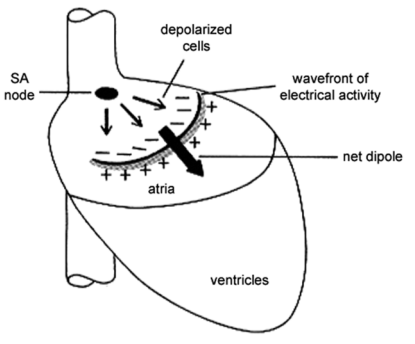
\includegraphics[scale=0.7]{img/heart_nature.PNG}
\caption{After conduction begins at the sinoatrial node, cells in the atria begin to depolarize. This creates an electrical wavefront that moves down toward the ventricles, with polarized cells at the front. The separation of charge results in a dipole across the heart (the large black arrow shows its direction) \cite{ecg1}.}
\label{fig:heart_nat}
\end{figure}


\section{ECG's history} \label{ecg_history}

The discovery of intrinsic electrical activity within the heart dates back to the 1840s. Carlo Matteucci, an Italian physicist, was the first to discover that each heartbeat is accompanied by an electrical current in 1842. Emil DuBois-Reymond, a German scientist, published the first action potential associated with muscular contraction not long after. In 1856, Rudolph von Koelliker and Heinrich Miller used a galvanometer to record the first cardiac action potential. Following that, Augustus D. Waller recorded the first human ECG after Gabriel Lippmann invented the capillary electrometer in the early 1870s. That first device is shown in Figure \ref{fig:Kapillarelektrometer}.

\begin{figure}[H]
\centering
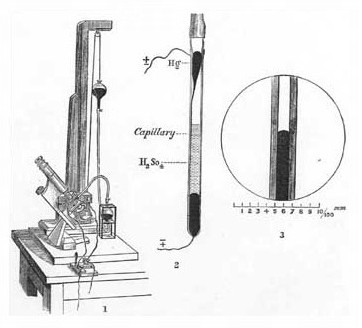
\includegraphics[scale=0.5]{img/Kapillarelektrometer.jpg}
\caption{Lippmann electrometer}
\label{fig:Kapillarelektrometer}
\end{figure}

Willem Einthoven's creation of the string galvanometer in 1901 was a key milestone in cardiac electrocardiography. The next year, he published the first ECG using his string galvanometer. Einthoven's string galvanometer consisted of a huge electromagnet with a thin silver-coated string stretched across it; electric currents passing through the thread caused the string to move from side to side in the electromagnet's magnetic field.


Einthoven made yet another significant addition to cardiac electrophysiology in 1912, when he discovered a mathematical link between the direction and size of the deflections recorded by the three limb leads. Einthoven's triangle is the name for this hypothesis. Before Frank Wilson described unipolar leads and the precordial lead configuration, the typical three-limb leads were used for three decades. The traditional Einthoven limb leads, as well as the precordial and unipolar limb, leads based on Wilson's work, make up the 12-lead ECG layout now in use.


This instrument was initially manufactured in 1905 by the Cambridge Scientific Instrument Company in London. Electrical impulses were sent from a hospital over a mile away to Einthoven's laboratory via a telephone cable. Bedside machines, on the other hand, were not available until the 1920s. The Sanborn Company produced a smaller version of the unit in 1935 that weighed only about 25 pounds.

\begin{figure}[H]
\centering
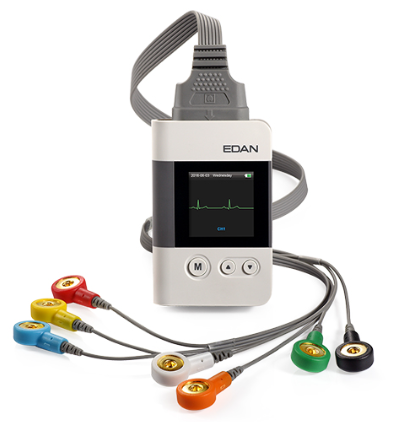
\includegraphics[scale=0.7]{img/holter_edan_ecg.PNG}
\caption{Holter-Edan ECG device}
\label{fig:holter_monitor}
\end{figure}

With Norman Jeff Holter's invention of the Holter monitor in 1949, the use of ECG in a nonclinical context became viable. The first iteration of this device was a 75-pound backpack that could record the ECG continually and send the signals via radio. The size of subsequent iterations of such devices has been drastically decreased, and the signal is now recorded digitally. Miniaturized devices now allow patients to be monitored for longer periods (typically 24 hours) to aid in the diagnosis of any rhythm or ischemic heart disease concerns. One of the latest versions of the ECG is the one appearing in Figure \ref{fig:holter_monitor}.

\section{The ECG Waveform} \label{ecg_waveform}

Signals of voltage versus time are created during the recording of an ECG, which are generally shown in millivolts (mV) vs seconds. Figure \ref{fig:ECG_waveform} depicts a typical Lead II ECG waveform. The negative electrode was placed on the right wrist and the positive electrode on the left ankle for this Lead II ECG recording. As a result, a series of peaks and waves can be seen, each of which corresponds to ventricular or atrial depolarization and repolarization, with each segment of the signal indicating a separate event in the cardiac cycle.

\begin{figure}[H]
\centering
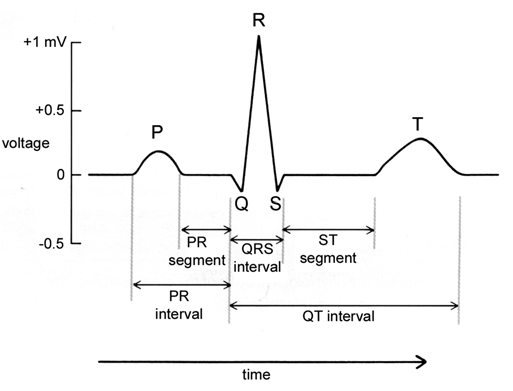
\includegraphics[scale=0.7]{img/ECG_waveform.PNG}
\caption{A typical ECG waveform for one cardiac cycle, measured from the Lead II position \cite{ecg1}.}
\label{fig:ECG_waveform}
\end{figure}
 
Three principal waveforms are recorded by the ECG (\ref{fig:ECG_waveform}):

\begin{itemize}
    \item The P-wave
    \item QRS complex
    \item T-wave.
\end{itemize}

The P-wave is created by depolarization of the atria, the QRS by depolarization of the ventricles, and the T-wave by repolarisation of the ventricles. In most people, these waveforms occur in a repeating rhythm called sinus rhythm, so called because it originates in the sinus node. In some people, a fourth waveform (not shown in the previous image) called a U-wave can be seen. This is usually seen at slower heart rates. The significance of the U-wave remains uncertain. Some authors think that it represents the late stages of ventricular repolarisation, while others describe it as a post-repolarisation phenomenon. U-wave abnormalities have been described in various disease states including ischaemic heart disease \cite{ecg2}.
 
 The depolarization of the sinoatrial node, which is positioned within the right atrium, starts the typical cardiac cycle. A conventional ECG will not detect this early firing because the node does not have enough cells to provide a measurable electrical potential. The right and left ventricles continue to depolarize after the P wave, resulting in the recordable QRS complex, which lasts about 100 milliseconds. The Q-wave is the initial negative deflection (if present), the R-wave is the largest positive deflection, and the S-wave is the smallest positive deflection \cite{ecg3}.
 
 
 The T-wave is usually the last potential in a cardiac cycle, followed by the P-wave of the next cycle, and so on. The ECG signal returns to baseline near the conclusion of ventricular contraction, and the ventricles repolarize after contraction. Atrial contractions have stopped and the atria are repolarizing at the same time as the QRS complex. Because the effects of this widespread atrial repolarization are obscured by the much larger volume of tissue engaged in ventricular depolarization, it is not generally detectable in an ECG \cite{ecg1}. 
 
 
\section{The 12-leads ECG} \label{12_lead_ecg}

An ECG lead is a recording of the heart's electrical activity as seen from one side. As a result, when we take a 12-lead ECG, we're recording cardiac electrical activity from 12 different angles \cite{ecg3}. Assume you're visiting a historic structure and taking images of it. If you snap 12 photos from different angles around the structure, each one will depict a distinct element, such as the front, sides, and back. They work together to provide a three-dimensional record of the structure's shape and appearance. Similarly, a 12-lead ECG creates a three-dimensional depiction of the heart's electrical activity.

\begin{figure}[H]
\centering
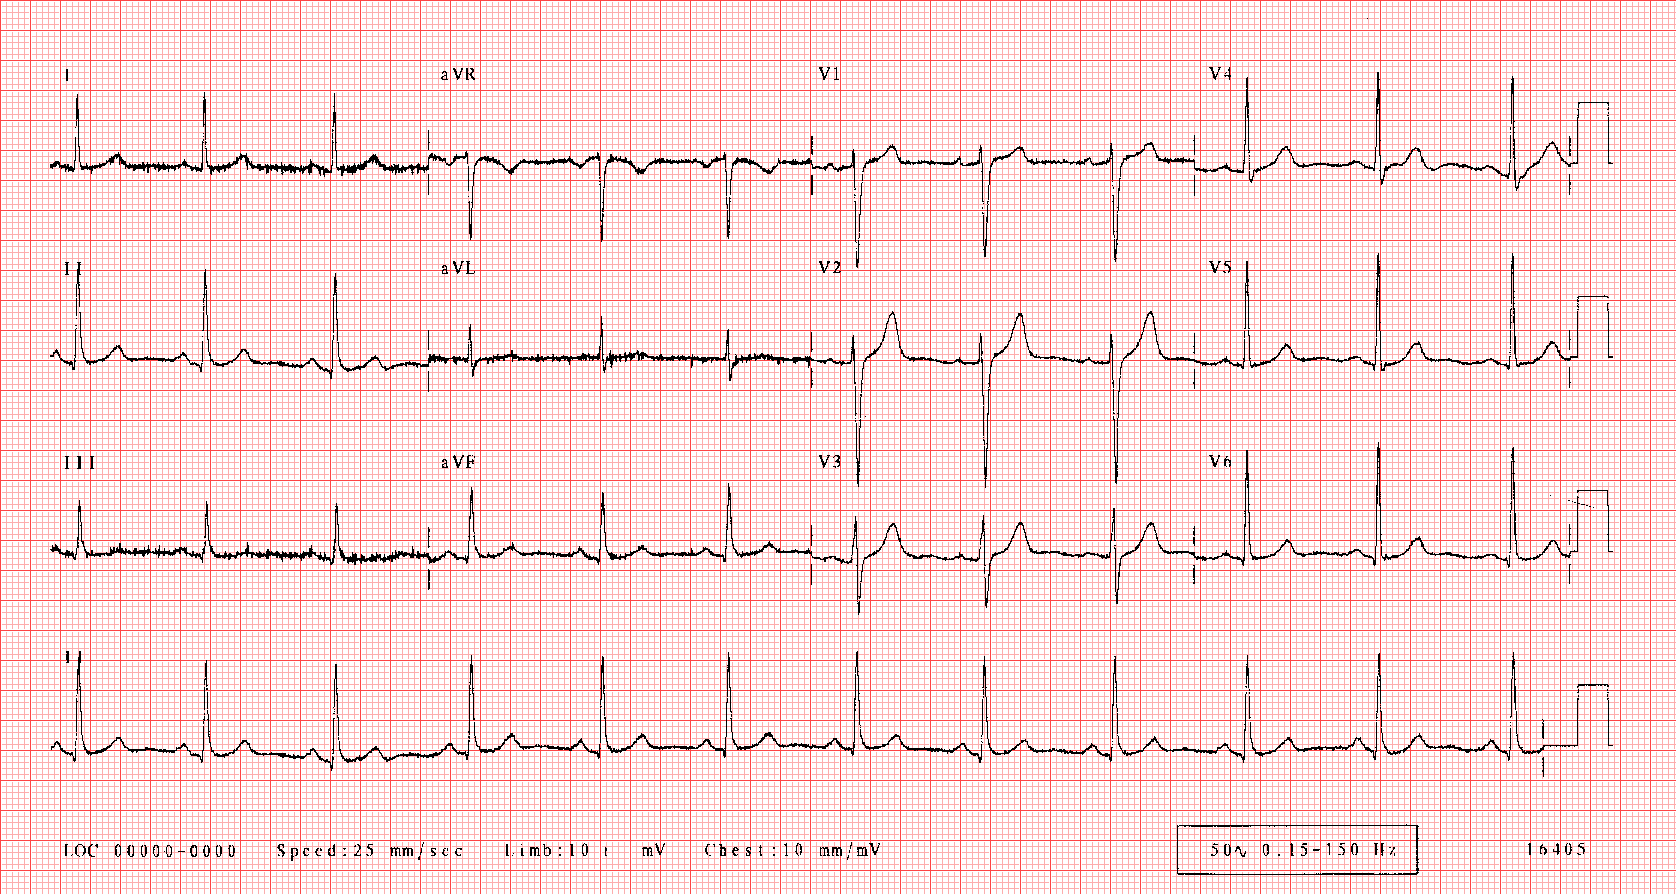
\includegraphics[scale=0.23]{img/normal_ecg.png}
\caption{12-leads normal ECG}
\label{fig:normal_ecg}
\end{figure}

Multiple images of the heart's electrical activity can be recorded depending on the type of machine utilized and the number of electrodes inserted. The usage of 12-lead ECG devices is common among healthcare professionals. Twelve separate electrical images of the heart are measured and recorded via a 12-lead ECG (Figure \ref{fig:normal_ecg}). In other words, it records the electrical activity of the heart as observed from 12 various angles. For example, Lead II monitors electrical activity as observed from the heart's inferior (diaphragmatic) surface. This lead is frequently used to measure heart rate \cite{basic_arryth}.

\section{Arrhythmias Types} \label{arrhythmias_types}

Analyzing arrhythmias is a difficult undertaking since every person on the planet has a unique ECG that differs from everyone else's, and one person's ECG can change dramatically from one second to the next. Memorizing some of the most common ECG patterns and attempting to recognize them in the future is insufficient. Pattern identification is a popular yet unintentional way of approaching arrhythmias via ECG analysis (\cite{arryth_types}). Often Arrhythmias are divided into two global categories:

\begin{enumerate}
    \item \textbf{Rhythmic}: Determined as a sequence of uneven beats
    \item \textbf{Morphological}: Made of abnormal single beat
\end{enumerate}

The work presented in the current thesis is focused on the first type of classification. Those arrhythmias have a categorization provided by SNOMED CT. The latter is the world's most complete and precise terminology package, with widespread acceptance around the world. It provides a common language for clinical IT systems, making data exchange between them easier, safer, and more accurate. It covers everything from processes and symptoms to clinical measurements, diagnosis, and drugs, and it's all in one place.

For the Physionet 2020 challenge only considered around 27 arrhythmias, which are the most frequently found in the ECG analysis. Nevertheless, in the following paragraphs, there is a deep explanation of all the possible arrhythmias. To see the complete list of categories it is possible to read the GitHub cited in \cite{github_arrhythmias}.

Arrhythmias are often divided into groups based on where the rhythm is initiated by the pacemaker. The following are the most prevalent sites, and consequently the primary arrhythmia categories:

\begin{enumerate}
    \item Sinus
    \item Atrial
    \item Junctional
    \item Ventricular
    \item AV Blocks
\end{enumerate}

\subsection{Sinus}

It is necessary to comprehend the 'benchmark' rhythm, or hemodynamically perfect rhythm, which is referred to as \textbf{Normal Sinus Rhythm} and sometimes abbreviated to \textbf{NSR}, in order to assess cardiac rhythms (Figure \ref{fig:nsr}). The following features must be present in order for a rhythm to be classified as Normal Sinus Rhythm:

\begin{table}[H]
\begin{center}
\begin{tabular}{||c || c||}
 \hline
\textbf{Characteristic} & \textbf{Status} \\ [0.4ex] 
 \hline\hline
Rhythm & Regular \\
\hline
Rate & 60-100/minute \\
\hline
p waves & Present, upright, symmetrical, one before every QRS \\
\hline
pri & .12-.20 seconds \\
\hline
QRS & .06-.10 seconds \\
\hline\hline
\end{tabular}
\end{center}
\caption{Characteristics of Normal Sinus Rhythm}
\label{table:nsr_characteristics}
\end{table}


\begin{figure}[H]
\centering
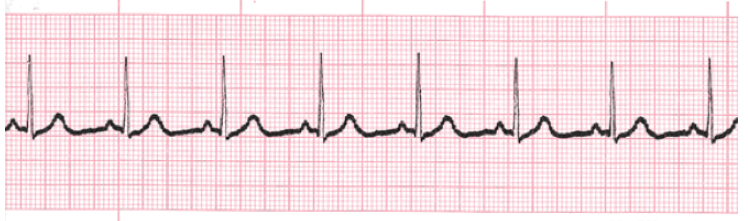
\includegraphics[scale=0.65]{img/NSR.png}
\caption{Normal Sinus Rhythm (\cite{arryth_types})}
\label{fig:nsr}
\end{figure}
 
\textbf{Sinus Bradycardia (SB)}: When a patient's heart rate falls below 60 beats per minute, they are said to be bradycardic. Slow heart rates can be seen in fit and active people who are usually asymptomatic. When a patient's heart rate falls below 60 beats per minute, critical care nurses must be ready to assess for decreasing cardiac output right away.

\begin{table}[H]
\begin{center}
\begin{tabular}{||c || c||}
 \hline
\textbf{Characteristic} & \textbf{Status} \\ [0.4ex] 
 \hline
 Rhythm & Regular \\
\hline\hline
Rate & < 60/minute \\
\hline
p waves & Present, upright, symmetrical, one before every QRS \\
\hline
pri & .12-.20 seconds \\
\hline
QRS & .06-.10 seconds \\
\hline\hline
\end{tabular}
\end{center}
\caption{Characteristics of Sinus Bradycardia}
\label{table:sb_characteristics}
\end{table}


 \begin{figure}[H]
\centering
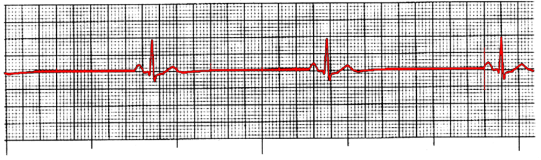
\includegraphics[scale=0.85]{img/SB.png}
\caption{Sinus Bradycardia (\cite{arryth_types})}
\label{fig:sb}
\end{figure}

\textbf{Sinus Tachycardia (STach)}: When a patient's heart rate exceeds 100 beats per minute, they are labelled tachycardic, though most people don't notice symptoms until their heart rate exceeds 150 beats per minute. At this point, a critical care nurse should look for signs and symptoms of decreased cardiac output (such as hypotension or a loss of consciousness).

\begin{table}[H]
\begin{center}
\begin{tabular}{||c || c||}
 \hline
\textbf{Characteristic} & \textbf{Status} \\ [0.4ex] 
 \hline\hline
 Rhythm & Regular \\
\hline
Rate & >100/minute \\
\hline
p waves & Present, upright, symmetrical, one before every QRS \\
\hline
pri & .12-.20 seconds \\
\hline
QRS & .06-.10 seconds \\
\hline\hline
\end{tabular}
\end{center}
\caption{Characteristics of Sinus Tachycardia}
\label{table:STach_characteristics}
\end{table}


 \begin{figure}[H]
\centering
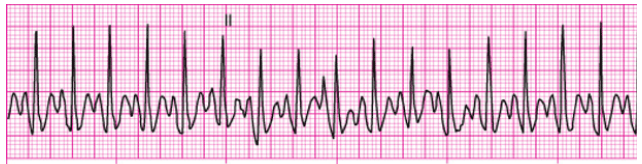
\includegraphics[scale=0.8]{img/STach.png}
\caption{Sinus Tachycardia (\cite{arryth_types})}
\label{fig:STach}
\end{figure}

\textbf{Sinus Arrhythmia (SA)}: This arrhythmia is typically benign and does not require any sort of treatment. It is seen in children and also in mechanically ventilated patients.

\begin{table}[H]
\begin{center}
\begin{tabular}{||c || c||}
 \hline
\textbf{Characteristic} & \textbf{Status} \\ [0.4ex] 
 \hline\hline
 Rhythm & Regular \\
\hline
Rate & 60-100/minute \\
\hline
p waves & Present, upright, symmetrical, one before every QRS \\
\hline
pri & .12-.20 seconds \\
\hline
QRS & .06-.10 seconds \\
\hline\hline
\end{tabular}
\end{center}
\caption{Characteristics of Sinus Arrhythmia}
\label{table:SA_characteristics}
\end{table}


 \begin{figure}[H]
\centering
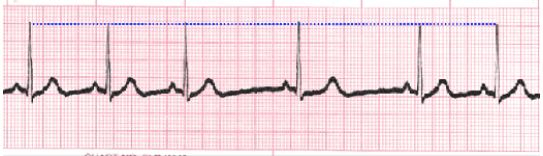
\includegraphics[scale=0.9]{img/SA.png}
\caption{Sinus Arrhythmia (\cite{arryth_types})}
\label{fig:SA}
\end{figure}

\textbf{Wandering Atrial Pacemaker (WAP)}: It can be a normal aberration associated with Ischemia. There is no treatment required.

\begin{table}[H]
\begin{center}
\begin{tabular}{||c || c||}
 \hline
\textbf{Characteristic} & \textbf{Status} \\ [0.4ex] 
 \hline\hline
 Rhythm & Regular \\
\hline
Rate & 60-100/minute \\
\hline
p waves & P waves vary in shape and size \\
\hline
pri & .12-.20 seconds \\
\hline
QRS & .06-.10 seconds \\
\hline\hline
\end{tabular}
\end{center}
\caption{Characteristics of Wandering Atrial Pacemaker}
\label{table:WAP_characteristics}
\end{table}


 \begin{figure}[H]
\centering
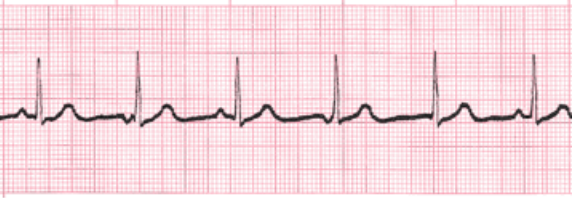
\includegraphics[scale=0.9]{img/WAP.png}
\caption{Wandering Atrial Pacemaker (\cite{arryth_types})}
\label{fig:WAP}
\end{figure}

\subsection{Atrial}

The rhythms that originate in the atrial will be examined in the following section. Premature atrial contractions, atrial flutter, atrial fibrillation, and supraventricular tachycardia are examples of these arrhythmias. The key characteristics of cardiac rhythms will be outlined, as well as nursing consequences and useful advice to help critical care nurses correctly interpret atrial arrhythmias.

\textbf{Premature Atrial Contractions (PAC)}: it can be a normal aberration,
Ischemia,  or a signal of atrial irritability. It can lead to more serious atrial rhythms.

\begin{table}[H]
\begin{center}
\begin{tabular}{||c || c||}
 \hline
\textbf{Characteristic} & \textbf{Status} \\ [0.4ex] 
 \hline\hline
 Rhythm & Early beat (PAC) causes rhythm to be irregular \\
\hline
Rate & Underlying rhythm usually 60-100/minute\\
\hline
p waves & P waves have different configuration than underlying rhythm \\
\hline
pri & .12-.20 seconds in underlying rhythm \\
\hline
QRS & .06-.10 seconds in underlying rhythm \\
\hline\hline
\end{tabular}
\end{center}
\caption{Characteristics of Premature Atrial Contractions}
\label{table:PAC_characteristics}
\end{table}

 \begin{figure}[H]
\centering
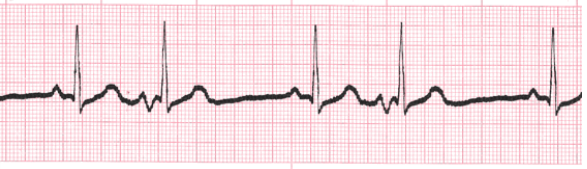
\includegraphics[scale=0.9]{img/PAC.png}
\caption{Premature Atrial Contractions (\cite{arryth_types})}
\label{fig:PAC}
\end{figure}

\textbf{Atrial Flutter (AFL)}: It is caused by electrolyte imbalance, Hypertension, Ischaemic heart disease, Congenital heart disease, and Rheumatic valve disease. Also after cardiac surgery.

\begin{table}[H]
\begin{center}
\begin{tabular}{||c || c||}
 \hline
\textbf{Characteristic} & \textbf{Status} \\ [0.4ex] 
 \hline\hline
 Rhythm & Regular or irregular \\
\hline
Rate & 60-100/minute (ventricular rate) 250-400 (atrial rate)\\
\hline
p waves & No p waves present. Flutter waves (F waves) or ‘sawtooth’ waves \\
\hline
pri & No pri since no p waves \\
\hline
QRS & .06-.10 seconds \\
\hline\hline
\end{tabular}
\end{center}
\caption{Characteristics of Atrial Flutter}
\label{table:AFL_characteristics}
\end{table}

 \begin{figure}[H]
\centering
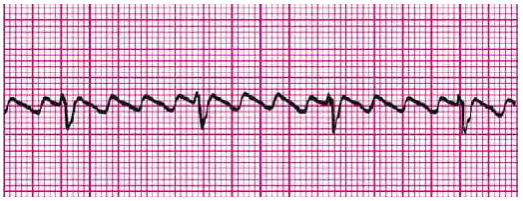
\includegraphics[scale=0.9]{img/AFL.png}
\caption{Atrial Flutter (\cite{arryth_types})}
\label{fig:AFL}
\end{figure}

\textbf{Atrial Fibrillation (AF)}: It is caused by Electrolyte imbalance, Hypertension, Ischaemic heart disease, Congenital heart disease, and Rheumatic valve disease. Also following cardiac surgery.

\begin{table}[H]
\begin{center}
\begin{tabular}{||c || c||}
 \hline
\textbf{Characteristic} & \textbf{Status} \\ [0.4ex] 
 \hline\hline
 Rhythm & Irregular \\
\hline
Rate & 60-100/minute (ventricular rate) >400/minute (atrial rate)\\
\hline
p waves & No p waves. Fibrillatory waves (f waves) \\
\hline
pri & No No pri since no p waves \\
\hline
QRS & .06-.10 seconds \\
\hline\hline
\end{tabular}
\end{center}
\caption{Characteristics of Atrial Fibrillation}
\label{table:AF_characteristics}
\end{table}

 \begin{figure}[H]
\centering
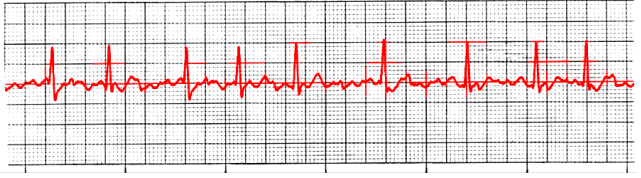
\includegraphics[scale=0.8]{img/AF.png}
\caption{Atrial Fibrillation (\cite{arryth_types})}
\label{fig:AF}
\end{figure}

\textbf{Supraventricular Tachycardia (SVT)}: It is caused by Congenital, heart disease, Emotional stress, Physical stress or exertion, Illegal drugs (i.e. Cocaine or ecstasy), Alcohol, Caffeine.

\begin{table}[H]
\begin{center}
\begin{tabular}{||c || c||}
 \hline
\textbf{Characteristic} & \textbf{Status} \\ [0.4ex] 
 \hline\hline
 Rhythm & Regular \\
\hline
Rate & 150-250/minute (atrial rate)\\
\hline
p waves & P waves may not be seen at higher rates \\
\hline
pri & .12-.20 seconds (if seen) \\
\hline
QRS & .06-.10 seconds \\
\hline\hline
\end{tabular}
\end{center}
\caption{Characteristics of Supraventricular Tachycardia}
\label{table:SVT_characteristics}
\end{table}

 \begin{figure}[H]
\centering
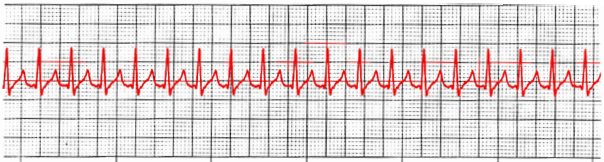
\includegraphics[scale=0.9]{img/SVT.png}
\caption{Supraventricular Tachycardia (\cite{arryth_types})}
\label{fig:SVT}
\end{figure}

\subsection{Junctional}

Junctional rhythms are temporary and non-lethal rhythms that originate in the AV node or junctional region. Inverted p waves are a typical feature of all junctional rhythms. Premature junctional contractions, junctional rhythm, and paroxysmal junctional tachycardia are among the rhythms covered in this section (\cite{arryth_types}).


\textbf{Premature Junctional Contraction (JPC)}: It is caused by Medication toxicity (i.e. digoxin), Ischemia. There is no treatment required.
Continue to observe for an increasing number of JPCs since this indicates
increasing AV node irritability.


\begin{table}[H]
\begin{center}
\begin{tabular}{||c || c||}
 \hline
\textbf{Characteristic} & \textbf{Status} \\ [0.4ex] 
 \hline\hline
 Rhythm & Early beat (PJC) causes the rhythm to be irregular \\
\hline
Rate & 60-100/minute (underlying rhythm)\\
\hline
p waves & P waves inverted or not seen in JPC \\
\hline
pri & Not applicable \\
\hline
QRS & .06-.10 seconds (in underlying rhythm) \\
\hline\hline
\end{tabular}
\end{center}
\caption{Characteristics of Premature Junctional Contraction}
\label{table:JPC_characteristics}
\end{table}

 \begin{figure}[H]
\centering
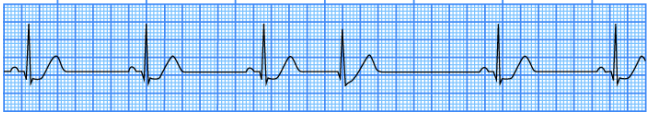
\includegraphics[scale=0.8]{img/JPC.png}
\caption{Premature Junctional Contraction (\cite{arryth_types})}
\label{fig:JPC}
\end{figure}


\textbf{Junctional Rhythm (AVJR)}: It is caused by Medication toxicity (i.e. digoxin) or ischemia. It is necessary to treat causes.


\begin{table}[H]
\begin{center}
\begin{tabular}{||c || c||}
 \hline
\textbf{Characteristic} & \textbf{Status} \\ [0.4ex] 
 \hline\hline
 Rhythm & Regular \\
\hline
Rate & <60/minute \\
\hline
p waves & P waves inverted or absent \\
\hline
pri & .12-.20 seconds \\
\hline
QRS & .06-.10 seconds \\
\hline\hline
\end{tabular}
\end{center}
\caption{Characteristics of Junctional Rhythm}
\label{table:AVJR_characteristics}
\end{table}

 \begin{figure}[H]
\centering
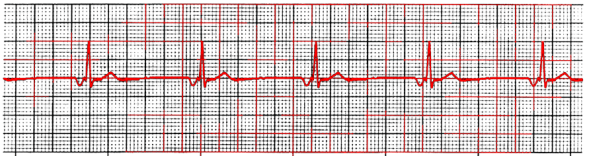
\includegraphics[scale=0.9]{img/AVJR.png}
\caption{Junctional Rhythm (\cite{arryth_types})}
\label{fig:AVJR}
\end{figure}


\textbf{Accelerated Junctional Rhythm (AJR)}: It is caused by Medication toxicity (i.e. digoxin) or ischemia. It is necessary to treat causes.

\begin{table}[H]
\begin{center}
\begin{tabular}{||c || c||}
 \hline
\textbf{Characteristic} & \textbf{Status} \\ [0.4ex] 
 \hline\hline
 Rhythm & Regular \\
\hline
Rate & 60-100/minute \\
\hline
p waves & P waves inverted or absent \\
\hline
pri & Not applicable \\
\hline
QRS & .06-.10 seconds \\
\hline\hline
\end{tabular}
\end{center}
\caption{Characteristics of Accelerated Junctional Rhythm}
\label{table:AJR_characteristics}
\end{table}

 \begin{figure}[H]
\centering
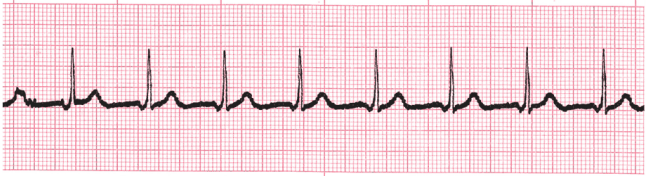
\includegraphics[scale=0.8]{img/AJR.png}
\caption{Accelerated Junctional Rhythm (\cite{arryth_types})}
\label{fig:AJR}
\end{figure}

\textbf{Paroxysmal Junctional Tachycardia (JT)}: It is caused by ischemia. Its treatment is the same as SVT.

\begin{table}[H]
\begin{center}
\begin{tabular}{||c || c||}
 \hline
\textbf{Characteristic} & \textbf{Status} \\ [0.4ex] 
 \hline\hline
 Rhythm & Regular \\
\hline
Rate & 150-250/minute \\
\hline
p waves & P waves inverted or absent (if seen) \\
\hline
pri & Not applicable \\
\hline
QRS & .06-.10 seconds \\
\hline\hline
\end{tabular}
\end{center}
\caption{Characteristics of Paroxysmal Junctional Tachycardia}
\label{table:JT_characteristics}
\end{table}

 \begin{figure}[H]
\centering
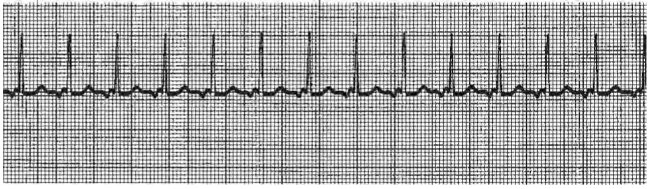
\includegraphics[scale=0.8]{img/JT.png}
\caption{Paroxysmal Junctional Tachycardia (\cite{arryth_types})}
\label{fig:JT}
\end{figure}


\subsection{Ventricular}

Premature ventricular contractions, ventricular tachycardia, and ventricular fibrillation are examples of ventricular rhythms that can be induced by irritability, as well as those that result from the failure of higher-level pacemakers. Irritability patients have significantly various treatment options and consequences.

\textbf{Premature Ventricular Contractions (PVC)}: It is caused by Ventricular irritability (i.e.hypoxemia, acid-base imbalance, medications, electrolyte imbalance).

\begin{table}[H]
\begin{center}
\begin{tabular}{||c || c||}
 \hline
\textbf{Characteristic} & \textbf{Status} \\ [0.4ex] 
 \hline\hline
 Rhythm & Early beat (PVC) causes the rhythm to be irregular \\
\hline
Rate & 60-100/minute (underlying rhythm) \\
\hline
p waves & None (in PVC) \\
\hline
pri & None (in PVC) \\
\hline
QRS & > .12 seconds (wide and bizzare) \\
\hline\hline
\end{tabular}
\end{center}
\caption{Characteristics of Premature Ventricular Contractions}
\label{table:PVC_characteristics}
\end{table}

 \begin{figure}[H]
\centering
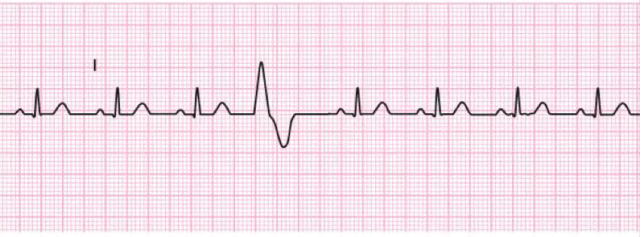
\includegraphics[scale=0.8]{img/PVC.png}
\caption{Premature Ventricular Contractions (\cite{arryth_types})}
\label{fig:PVC}
\end{figure}

\textbf{Ventricular Tachycardia (VTach)}: It is caused by Ventricular irritability (i.e.hypoxemia, acid-base imbalance, medications, electrolyte
imbalance).

\begin{table}[H]
\begin{center}
\begin{tabular}{||c || c||}
 \hline
\textbf{Characteristic} & \textbf{Status} \\ [0.4ex] 
 \hline\hline
 Rhythm & Regular \\
\hline
Rate & 150-250/min \\
\hline
p waves & None  \\
\hline
pri & None  \\
\hline
QRS & > .12 seconds (wide and bizzare) \\
\hline\hline
\end{tabular}
\end{center}
\caption{Characteristics of Premature Ventricular Contractions}
\label{table:VTach_characteristics}
\end{table}

 \begin{figure}[H]
\centering
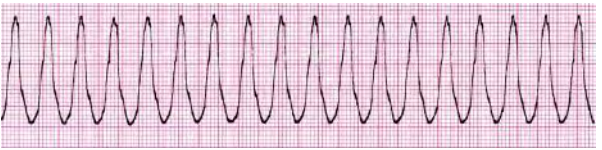
\includegraphics[scale=0.8]{img/VTach.png}
\caption{Premature Ventricular Contractions (\cite{arryth_types})}
\label{fig:VTach}
\end{figure}

\textbf{Ventricular Fibrillation (VF)}: It is caused by Ventricular irritability (i.e.hypoxemia, acid-base imbalance, medications, electrolyte
imbalance).

\begin{table}[H]
\begin{center}
\begin{tabular}{||c || c||}
 \hline
\textbf{Characteristic} & \textbf{Status} \\ [0.4ex] 
 \hline\hline
 Rhythm & Irregular and chaotic \\
\hline
Rate & Cannot calculate \\
\hline
p waves & None  \\
\hline
pri & None  \\
\hline
QRS & None \\
\hline\hline
\end{tabular}
\end{center}
\caption{Characteristics of Ventricular Fibrillation}
\label{table:VF_characteristics}
\end{table}

 \begin{figure}[H]
\centering
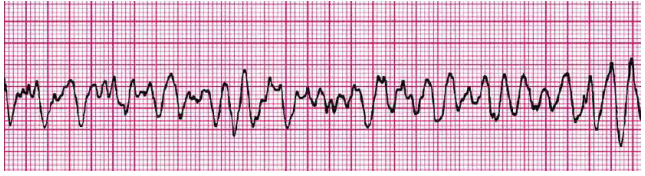
\includegraphics[scale=0.8]{img/VF.png}
\caption{Ventricular Fibrillation (\cite{arryth_types})}
\label{fig:VF}
\end{figure}

\textbf{Idioventricular Rhythm (IR)}: It is caused by Ischemia, reperfusion post thrombolytics.

\begin{table}[H]
\begin{center}
\begin{tabular}{||c || c||}
 \hline
\textbf{Characteristic} & \textbf{Status} \\ [0.4ex] 
 \hline\hline
 Rhythm & Regular \\
\hline
Rate & <40/minute \\
\hline
p waves & No p waves  \\
\hline
pri & No pri  \\
\hline
QRS & > .12 seconds (wide and bizarre) \\
\hline\hline
\end{tabular}
\end{center}
\caption{Characteristics of Idioventricular Rhythm}
\label{table:IR_characteristics}
\end{table}

 \begin{figure}[H]
\centering
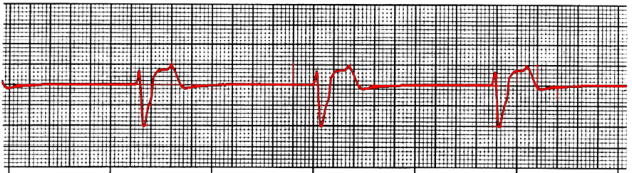
\includegraphics[scale=0.8]{img/IR.png}
\caption{Idioventricular Rhythm}
\label{fig:IR}
\end{figure}


\subsection{AV Blocks}

Electrical conduction failure via the myocardium is characterized by atrioventricular (AV) blockages. Because AV blockages are linked to severe risk worsening or haemodynamic impairment, the critical care nurse must recognize and treat them as soon as possible. 1st-degree heart block, 2nd-degree heart block (Mobitz type 1 or Wenkebach), and 3rd-degree heart block are all types of AV block (complete heart block).  (\cite{arryth_types})

\textbf{First Degree AV Block (IAVB)}: It is caused by AV nodal disease, Enhanced vagal tone (i.e. athletes), Myocarditis, Following Myocardial Infarction, Electrolyte disturbances, Medications (i.e. Calcium channel blockers, Beta blockers).

\begin{table}[H]
\begin{center}
\begin{tabular}{||c || c||}
 \hline
\textbf{Characteristic} & \textbf{Status} \\ [0.4ex] 
 \hline\hline
 Rhythm & Regular \\
\hline
Rate & 60-100/minute \\
\hline
p waves & P waves normal  \\
\hline
pri & >.20 seconds     \\
\hline
QRS & .06-.10 seconds \\
\hline\hline
\end{tabular}
\end{center}
\caption{Characteristics of First Degree AV Block}
\label{table:IAVB_characteristics}
\end{table}

 \begin{figure}[H]
\centering
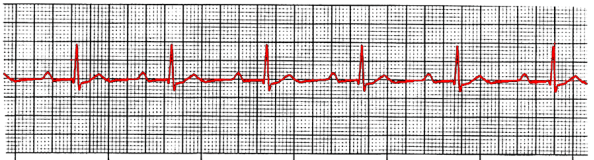
\includegraphics[scale=0.8]{img/IAVB.png}
\caption{First Degree AV Block (\cite{arryth_types})}
\label{fig:IAVB}
\end{figure}


\textbf{Second Degree Type I (IIAVB)}: It is caused by Ischemia. Usually benign, with no treatment required. If a patient becomes haemodynamically compromised interventions for bradycardia should be considered.


\begin{table}[H]
\begin{center}
\begin{tabular}{||c || c||}
 \hline
\textbf{Characteristic} & \textbf{Status} \\ [0.4ex] 
 \hline\hline
 Rhythm & Regular or slightly irregular \\
\hline
Rate & 60-100/minute \\
\hline
p waves & P waves normal  \\
\hline
pri & Progressively gets longer until a beat is dropped     \\
\hline
QRS & .06-.10 seconds \\
\hline\hline
\end{tabular}
\end{center}
\caption{Characteristics of Second Degree Type I}
\label{table:IIAVB_characteristics}
\end{table}

 \begin{figure}[H]
\centering
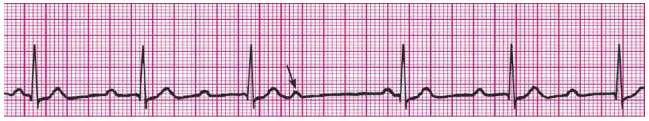
\includegraphics[scale=0.8]{img/IIAVB.png}
\caption{Second Degree Type I (\cite{arryth_types})}
\label{fig:IIAVB}
\end{figure}


